\let\negmedspace\undefined
\let\negthickspace\undefined
\documentclass[article]{IEEEtran}
\usepackage[a5paper, margin=10mm, onecolumn]{geometry}
%\usepackage{lmodern} % Ensure lmodern is loaded for pdflatex
\usepackage{tfrupee} % Include tfrupee package

\setlength{\headheight}{1cm} % Set the height of the header box
\setlength{\headsep}{0mm}     % Set the distance between the header box and the top of the text

\usepackage{gvv-book}
\usepackage{gvv}
\usepackage{cite}
\usepackage{amsmath,amssymb,amsfonts,amsthm}
\usepackage{algorithmic}
\usepackage{graphicx}
\usepackage{textcomp}
\usepackage{xcolor}
\usepackage{txfonts}
\usepackage{listings}
\usepackage{enumitem}
\usepackage{mathtools}
\usepackage{gensymb}
\usepackage{comment}
\usepackage[breaklinks=true]{hyperref}
\usepackage{tkz-euclide} 
\usepackage{listings}                                       
\def\inputGnumericTable{}                                 
\usepackage[latin1]{inputenc}                                
\usepackage{color}                                            
\usepackage{array}                                            
\usepackage{longtable}                                       
\usepackage{calc}                                             
\usepackage{multirow}                                         
\usepackage{hhline}                                           
\usepackage{ifthen}                                           
\usepackage{lscape}

\renewcommand{\thefigure}{\theenumi}
\renewcommand{\thetable}{\theenumi}
\setlength{\intextsep}{10pt} % Space between text and floats

\numberwithin{figure}{enumi}
\renewcommand{\thetable}{\theenumi}

% Marks the beginning of the document
\begin{document}
\bibliographystyle{IEEEtran}

\title{2009-EE-1-12}
\author{EE24BTECH11035 - KOTHAPALLI AKHIL}
{\let\newpage\relax\maketitle}

\begin{enumerate}
\item The pressure coil of a dynamometer type wattmeter is  
\begin{enumerate}
\item highly inductive
\item highly resistive
\item purely resistive
\item purely inductive
\end{enumerate}

\item The measurement system shown in the figure uses three sub-systems in cascade whose gains are specified as $G_1$, $G_2$, and $\frac{1}{G_3}$. The relative small errors associated with each respective subsystem $G_1$, $G_2$, and $G_3$ are $\epsilon_1$, $\epsilon_2$, and $\epsilon_3$. The error associated with the output is:  
\begin{figure}[!ht]
\centering
\resizebox{0.4\textwidth}{!}{%
\begin{circuitikz}
\tikzstyle{every node}=[font=\LARGE]
\draw [short] (12.25,14.5) .. controls (10.25,11.25) and (10.5,11.75) .. (7.25,11.5);
\draw [short] (7.25,11) .. controls (11.75,11.75) and (9,10) .. (8.5,9.25);
\draw [short] (13.25,14.25) -- (9,8.75);
\draw [ rotate around={-37:(11.75, 11.875)}] (12,14.25) rectangle (11.5,9.5);
\draw [short] (12,11.75) -- (14,11.75);
\draw [short] (12.5,12.5) .. controls (12.75,12.25) and (12.75,12.25) .. (12.75,11.75);
\draw [->, >=Stealth] (12.5,14) -- (13.25,15.25);
\draw [->, >=Stealth] (9,9.25) -- (8,8.25);
\draw [short] (9,9.75) -- (9.5,9.5);
\draw [short] (12,14) -- (12.75,13.5);
\draw [dashed] (7.75,12) -- (7.75,10.75);
\draw [->, >=Stealth] (6,11.25) -- (7.5,11.25);
\node [font=\LARGE] at (8,12.25) {1};
\node [font=\LARGE] at (11.5,14.5) {2};
\node [font=\LARGE] at (9.75,9) {3};
\node [font=\LARGE] at (12.5,11) {plate};
\node [font=\LARGE] at (13.25,12.5) {$\theta$};
\end{circuitikz}
}%

\label{fig:my_label}
\end{figure}

\begin{enumerate}
\item $\epsilon_1 + \epsilon_2 + \frac{1}{\epsilon_3}$
\item $\frac{\epsilon_1 \cdot \epsilon_2}{\epsilon_3}$
\item $\epsilon_1 + \epsilon_2 - \epsilon_3$
\item $\epsilon_1 + \epsilon_2 + \epsilon_3$
\end{enumerate}

\item The following circuit has a source voltage $V_s$ as shown in the graph. The current through the circuit is also shown. The element connected between $a$ and $b$ could be:  
% f3.tex
\begin{figure}[!ht]
    \centering
    \resizebox{0.5\textwidth}{!}{%
        \begin{circuitikz}
            \tikzstyle{every node}=[font=\large]
          
            % Removed grid line from here
            \draw  (6.5,11) rectangle (8.25,10);
            \draw [short] (6.5,10.5) -- (4.75,10.5);
            \draw [short] (8.25,10.5) -- (9.75,10.5);
            \draw (4.75,10.5) to[american voltage source,l={ \large $V_s$}] (4.75,8);
            \draw (9.75,10.5) to[R,l={ \large 10K}] (9.75,8);
            \draw (9.75,8) to[short] (4.75,8);
            \node [font=\large] at (6.25,10.75) {$a$};
            \node [font=\large] at (8.5,10.75) {$b$};
        \end{circuitikz}
    }%
    \label{fig:my_label}
\end{figure}

\begin{figure}[ht]
\centering
    \begin{minipage}[b]{0.3\linewidth} % Decrease the width to make the images smaller
        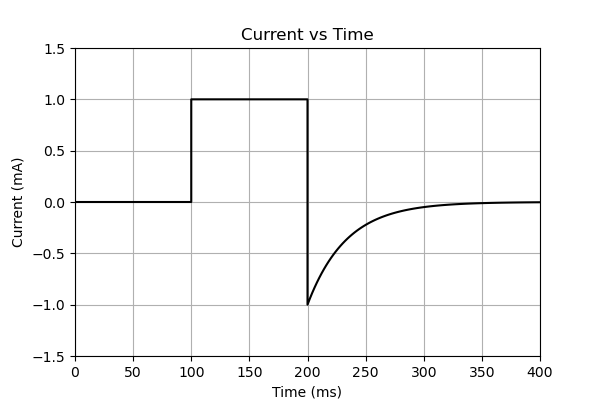
\includegraphics[width=0.9\linewidth]{graphs/Figure_1.png} % Adjust the width of the image 
    \end{minipage}
    \hspace{0.02\linewidth} % Smaller horizontal space between the figures
    \begin{minipage}[b]{0.3\linewidth} % Decrease the width to make the images smaller
        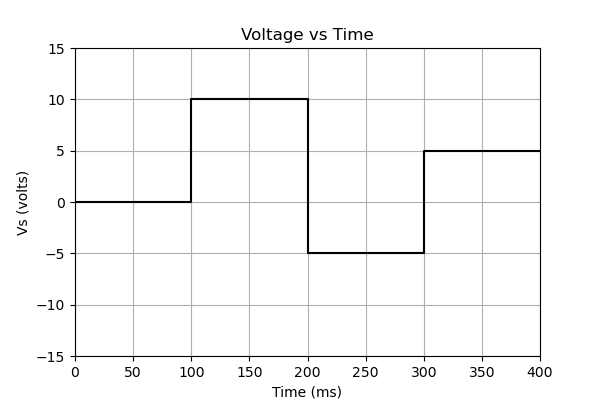
\includegraphics[width=0.9\linewidth]{graphs/Figure_2.png} % Adjust the width of the image 
    \end{minipage}
\end{figure}
\begin{enumerate}
\item 

\resizebox{0.3\textwidth}{!}{%
\begin{circuitikz}
\tikzstyle{every node}=[font=\LARGE]
\draw [->, >=Stealth] (7.75,8.5) -- (15.5,8.5);
\draw [->, >=Stealth] (8,8.25) -- (8,12.75);
\draw [short] (8,11.75) .. controls (9.25,10.5) and (9.25,6.25) .. (11.5,10);
\draw [short] (11.5,10) .. controls (12,12) and (12.5,10.75) .. (13,10);
\draw [short] (13,10) .. controls (13.75,8.75) and (13.5,8.25) .. (14.75,10);
\node [font=\LARGE] at (7.25,10.75) {$P(r)$};
\node [font=\LARGE] at (10.5,8.25) {$r/a_0$};
\end{circuitikz}
}%

\label{fig:my_label}

\item \
\resizebox{0.2\textwidth}{!}{%
\begin{circuitikz}
\tikzstyle{every node}=[font=\small]
\draw (7.75,13.75) to[C] (9.75,13.75);
\node [font=\small, rotate around={-360:(0,0)}] at (7.5,13.75) {A};
\node [font=\small] at (10,13.75) {B};
\end{circuitikz}
}%

\label{fig:my_label}


\item 

\resizebox{0.3\textwidth}{!}{%
\begin{circuitikz}
\tikzstyle{every node}=[font=\LARGE]
\draw [->, >=Stealth] (7.75,6.5) -- (7.75,13);
\draw [->, >=Stealth] (7,7.25) -- (13.75,7.25);
\draw [short] (7.75,11.75) .. controls (8,8.25) and (8.25,7.5) .. (9.75,7.25);
\node [font=\LARGE] at (6.75,9.75) {$P(r)$};
\node [font=\LARGE] at (10,6.75) {$r/a_0$};
\end{circuitikz}
}%

\label{fig:my_label}

\item 

\resizebox{0.3\textwidth}{!}{%
\begin{circuitikz}
\tikzstyle{every node}=[font=\LARGE]
\draw [->, >=Stealth] (7.75,6.5) -- (7.75,13);
\draw [->, >=Stealth] (7.25,7.25) -- (18,7.25);
\draw [short] (7.75,7.25) .. controls (12.5,18.5) and (11.75,7.25) .. (15.75,7.25);
\node [font=\LARGE] at (6.75,9.75) {$P(r)$};
\node [font=\LARGE] at (10,6.75) {$r/a_0$};
\end{circuitikz}
}%

\label{fig:my_label}

\end{enumerate}



\item The two inputs of a CRO are fed with two stationary periodic signals. In the X-Y mode, the screen shows a figure which changes from ellipse to circle and back to ellipse with its major axis changing orientation slowly and repeatedly. The following inference can be made from this:

\begin{enumerate}
\item The signals are not sinusoidal
\item The amplitudes of the signals are very close but not equal
\item The signals are sinusoidal with their frequencies very close but not equal
\item There is a constant but small phase difference between the signals
\end{enumerate}

\item The increasing order of speed of data access for the following devices is:

(i) Cache Memory \\
(ii) CDROM \\
(iii) Dynamic RAM \\
(iv) Processor Registers \\
(v) Magnetic Tape \\

\begin{enumerate}
\item (v), (ii), (iii), (iv), (i)
\item (v), (iii), (ii), (i), (iv)
\item (ii), (i), (iii), (iv), (v)
\item (v), (iv), (i), (iii), (ii)
\end{enumerate}

\item A field excitation of $20 \, \text{A}$ in a certain alternator results in an armature current of $400 \, \text{A}$ in short circuit and a terminal voltage of $2000 \, \text{V}$ on open circuit. The magnitude of the internal voltage drop within the machine at a load current of $200 \, \text{A}$ is:

\begin{enumerate}
\item $1 \, \text{V}$
\item $10 \, \text{V}$
\item $100 \, \text{V}$
\item $1000 \, \text{V}$
\end{enumerate}

\item The current through the $2 \, \text{k}\Omega$ resistance in the circuit shown is:
% f1.tex
\begin{figure}[!ht]
    \centering
    \resizebox{0.5\textwidth}{!}{% % Adjusted width from 1\textwidth to 0.5\textwidth
        \begin{circuitikz}
            \tikzstyle{every node}=[font=\small]
            \draw (2.75,21) to[R,l={ \small 1K}] (4.75,21);
            \draw (4.75,21) to[R] (6.75,21);
            \draw (2.75,19.25) to[R,l={ \small 1K}] (4.75,19.25);
            \draw (4.75,19.25) to[R,l={ \small 1K}] (6.75,19.25);
            \draw (4.75,21) to[R,l={ \small 1K}] (6.75,21);
            \draw [line width=0.5pt] (4.75,21) to[R] (4.75,19.25);
            \draw [line width=0.5pt] (6.75,21) to[short] (6.75,19.25);
            \draw [line width=0.5pt] (2.75,21) to[short] (2.75,19.25);
            \draw [line width=0.5pt] (1.5,20.25) to[short] (2.75,20.25);
            \draw [line width=0.5pt] (6.75,20.25) to[short] (7.75,20.25);
            \draw [line width=0.5pt] (1.5,20.25) to[short] (1.5,17.75);
            \draw [line width=0.5pt] (7.75,20.25) to[short] (7.75,17.75);
            \draw (1.5,17.75) to[battery1,l=$6V$] (7.75,17.75);
            \node [font=\normalsize] at (2.5,20.5) {A};
            \node [font=\normalsize] at (7,20.5) {B};
            \node [font=\normalsize] at (4.75,21.25) {C};
            \node [font=\small] at (4.75,19) {D};
        \end{circuitikz}
    }
    
    \label{fig:my_label}
\end{figure}

\begin{enumerate}
\item $0 \, \text{mA}$
\item $1 \, \text{mA}$
\item $2 \, \text{mA}$
\item $6 \, \text{mA}$
\end{enumerate}

\item Out of the following plant categories, the base load power plants are:

(i) Nuclear \\
(ii) Run-of-river \\
(iii) Pump Storage \\
(iv) Diesel \\

\begin{enumerate}
\item (i) and (ii)
\item (ii) and (iii)
\item (i), (ii) and (iv)
\item (i), (iii) and (iv)
\end{enumerate}

\item For a fixed value of complex power flow in a transmission line having a sending end voltage $V$, the real power loss will be proportional to:

\begin{enumerate}
\item $V$
\item $V^2$
\item $\frac{1}{V^2}$
\item $\frac{1}{V}$
\end{enumerate}

\item How many 200W/220V incandescent lamps connected in series would consume the same total power as a single 100W/220V incandescent lamp?

\begin{enumerate}
\item not possible
\item 4
\item 3
\item 2
\end{enumerate}

\item A Linear Time Invariant system with an impulse response $h(t)$ produces output $y(t)$ when input $x(t)$ is applied. When the input $x(t - \tau)$ is applied to a system with impulse response $h(t - \tau)$, the output will be

\begin{enumerate}
\item $y(t)$
\item $y(2(t - \tau))$
\item $y(t - \tau)$
\item $y(t - 2\tau)$
\end{enumerate}

\item The nature of feedback in the opamp circuit shown is
\begin{figure}[!ht]
    \centering
    \resizebox{0.3\textwidth}{!}{%

\begin{circuitikz}

\tikzstyle{every node}=[font=\small]
\draw (9.75,12.5) node[op amp,scale=1] (opamp2) {};
\draw (opamp2.+) to[short] (8.25,12);
\draw  (opamp2.-) to[short] (8.25,13);
\draw (10.95,12.5) to[short](11.25,12.5);
\draw (6.75,13) to[R] (8.25,13);
\draw (6.75,13) to (6.75,12.5) node[ground]{};
\draw (8.25,13) to[short] (8.25,14.5);
\draw (8.25,14.5) to[short] (11.75,14.5);
\draw (11.75,14.5) to[R] (11.75,12.5);
\draw (11.25,12.5) to[short, -o] (13,12.5) ;
\draw (9.75,13.75) to[short] (9.75,13);
\draw (9.75,12) to[short] (9.75,11.25);
\draw (8.25,12) to[sinusoidal voltage source, sources/symbol/rotate=auto] (8.25,10.5);
\draw (8.25,10.5) to (7.75,10.5) node[ground]{};
\node [font=\small] at (7.5,13.5) {1 k$\Omega$};
\node [font=\small] at (9.75,14) {+6V};
\node [font=\small] at (9.75,11) {-6V};
\node [font=\small] at (12.5,13.5) {2 k$\Omega$};
\node [font=\small] at (13.25,12) {V(out)};
\node [font=\small] at (7.5,11) {V(in)};
\end{circuitikz}
}%
\end{figure}

\begin{enumerate}
\item Current - Current feedback
\item Voltage - Voltage feedback
\item Current - Voltage feedback
\item Voltage - Current feedback
\end{enumerate}

\end{enumerate}
\end{document}

